% TODO: vllt dieses kapitel auf dateien teilen, is ziemlich lang
In diesem Kapitel werden die zum Verständnis der Implementierung benötigten theoretischen, sowie technischen Grundlagen beschrieben. Dabei werden primär die Funktionalität von WebRTC an sich, als auch die damit verbundenen Signal-Mechanismen und Infrastrukturen behandelt. Zudem wird ein kurzer Überblick über die Cloud-Computing Plattform Microsoft Azure gegeben, da diese als prototypische Deployment-Plattform verwendet wird.

\section{Echtzeitanwendungen}
Unter den Begriff Echtzeitanwendung fällt prinzipiell jede Anwendung, deren von Nutzern ausgelöste Ereignisse nur gewisse, in der Regel für den Nutzer nicht wahrnehmbare Verzögerungen aufweisen dürfen. Ein Beispiel für Echtzeitanwendungen sind Audio- und Videokommunikationsprogramme. Die Audio- und Videodaten müssen schnellstmöglich zwischen den Teilnehmern eines Anrufs ausgetauscht werden, um den Eindruck zu vermitteln, dass die Gesprächsteilnehmer direkt miteinander sprechen. Spricht zum Beispiel eine Person, so muss der Ton zur nahezu gleichen Zeit bei allen anderen Personen, welche dem Anruf teilhaben, ankommen.

\section{WebRTC}
Bei \ac{WebRTC} handelt es sich um einen Quelloffenen Standard zur Echtzeitkommunikation zwischen Browsern. Im Gegensatz zu weiteren Echtzeitstandards, wie zum Beispiel WebSockets, setzt \acs{WebRTC} nicht auf ein Client-Server Modell. Stattdessen ermöglicht der Standard es Browsern, welche den \acs{WebRTC} Standard unterstützen, sich ohne zusätzliche Software oder Plugins direkt miteinander zu verbinden. Der Datenaustausch findet somit direkt zwischen den Browsern -- den sogenannten Peers -- statt, ohne dass die Daten zusätzlich über einen Server weitergeleitet werden müssen. Dies führt in der Regel zu geringeren Latenzen, sowie Kostenersparnissen durch weniger Serverlast.\par

Der Standard wird von einer Arbeitsgruppe des \acs{W3C}, der \acs{WebRTC} Working Group (dt. WebRTC Arbeitsgruppe) entwickelt und erhalten. Insgesamt 18 Organisationen sind in der WebRTC Arbeitsgruppe vertreten, unter anderem Microsoft, Google, Mozilla, Cisco und Apple \cite{webRTCWorkingGroup}.\par

\subsection{Aufbau von WebRTC}
WebRTC ist kein proprietärer, einzelner und zusammenhängender Standard, sondern eine Ansammlung bereits existierender Protokolle, Technologien und Standards, welche unter anderem den Aufbau von Verbindungen, Audio- und Videoübertragung, sowie Datenübertragung regeln.\par

\begin{figure}[h]
\centering
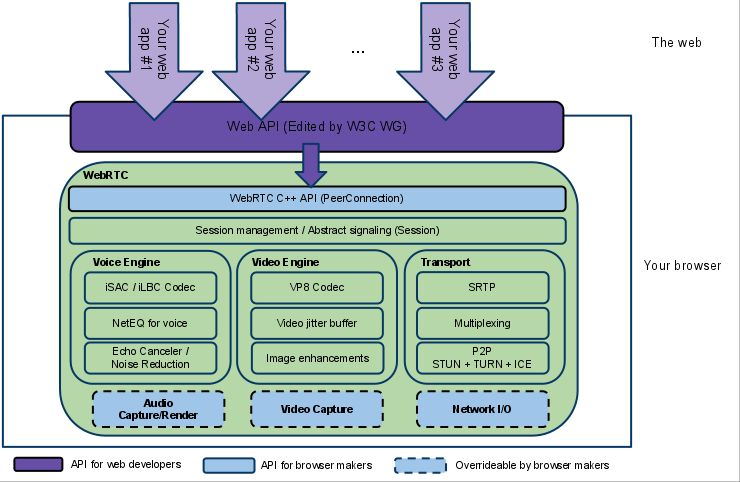
\includegraphics[width=0.95\textwidth]{bilder/webrtc-diagram.png}
\caption{Diagramm der WebRTC-Architektur.}
\source{\url{https://webrtc.github.io/webrtc-org/architecture/}}
\end{figure}

Wie dem Architekturdiagramm in Abbildung 2.1 zu entnehmen, gliedert sich WebRTC primär in eine Web-\acs{API} und das \acs{WebRTC}-Framework. Hinzu kommen Signalisierungsmechanismen, welche zum Aufbau einer Verbindung benötigt werden. Diese sind nicht durch den WebRTC-Standard vorgeschrieben. Es ist dem Entwickler überlassen, wie die Signalisierung letztendlich implementiert wird -- es muss lediglich möglich sein, Daten zur Sitzunsinitialisierung zwischen jeweils zwei Peers auszutauschen.\par

\subsubsection*{Web-API}
Die Web-\acs{API} dient dabei zur Entwicklung von Browserbasierten Webanwendungen, und setzt sich aus einer Reihe an JavaScript Schnittstellen zusammen. Diese Schnittstellen können auf das unterliegende Framework zugreifen, und ermöglichen zum Beispiel das Erstellen von Verbindungen, Datenkanälen und Video-Streams. Primär werden dabei die folgenden Schnittstellen verwendet:

\begin{itemize}
  \item Die \textbf{RTCPeerConnection}-Schnittstelle repräsentiert eine WebRTC-Verbindung zwischen dem lokalen Browser (Local-Peer), und einem externen Browser (Remote-Peer) \cite{rtcpeerconnection}. Die Signalisierungsmechanismen folgen dabei dem \ac{JSEP}, die Verbindung selbst wird via dem \ac{ICE} Framework hergestellt.
  
  \item Ein \textbf{RTCDataChannel} ist ein, von der RTCPeerConnection erstellter, bidirektionaler Datenkanal, welcher den Austausch von arbitraren Nachrichten zwischen Browsern ermöglicht. Eine RTCPeerConnection kann mehrere Datenkanäle besitzen. Zum Datenaustausch wird das \ac{SCTP} verwendet \cite{rtcpeerconnection}.
  
  \item Die \textbf{MediaStream}-\acs{API} dient dazu, Audio- und Videosignale eines Gerätes abzurufen. Dabei wird ein Datenstrom erzeugt, welcher in Echtzeit an externe Browser gesendet werden kann. Dazu wird das \ac{RTP}, beziehungsweise das \ac{SRTP} verwendet. Da Audio- und Videoübertragung für diese Arbeit nicht relevant sind, wird auf diese Protokolle nicht weiter eingegangen.
\end{itemize}

\subsubsection*{WebRTC Framework}
Das \acs{WebRTC}-Framework gliedert sich primär in Audio- Video- und Übertragungssysteme. Die Audio- und Videosysteme befassen sich dabei unter anderem mit der Abfrage von Audiodaten des Gerätemikrofons, sowie Videodaten über eine Kamera, welche an das Gerät angeschlossen ist. Zudem sind diese Systeme für die en- und decodierung von Audio- und Videodaten auf Basis verschiedener \glqq{}Codecs\grqq{} zuständig. Auf diese wird hier nicht weiter eingegangen.\par

Die Transportsysteme umfassen Protokolle und Systeme, um Sitzungen zwischen Peers aufzubauen, und Daten zwischen den Peers zu versenden. Die Sitzungskomponenten basieren dabei auf \glqq{}libjingle\grqq{}, einem Quelloffenen C++ \ac{SDK}, welches das Erstellen von Peer-To-Peer Sitzungen ermöglicht. Hinzu kommen Protkolle wie \acs{STUN}, \acs{TURN} und \acs{ICE}, welche im Unterpunkt \glqq{}Protokolle\grqq{} näher erläutert werden.

\subsection{Protokolle und Frameworks}
Die mit der Implementierung zusammenhängenden Protokolle werden im Fogenden näher erläutert -- sowohl deren Funktionalität, als auch deren Zusammenspiel untereinander.\par

\subsubsection{JSEP}
Die Signalisierungsebene einer \acs{WebRTC}-Anwendung ist nicht vom \acs{WebRTC}-Standard definiert, damit verschiedene Applikationen mitunter verschiedene Signalisierungsprotkolle, wie zu Beispiel das \acf{SIP}, oder ein proprietäres Protokoll nutzen können.\par

Das \acf{JSEP} erlaubt es einem Entwickler, die volle Kontrolle über die unterliegende Zustandsmaschine des Signalisierungsprozesses zu haben, welche die Initialisierung einer Sitzung kontrolliert. Damit werden die Signalisierungs- und Datenübertragungsebene effektiv voneinander getrennt. Eine Sitzung wird immer zwischen zwei Endpunkten etabliert, einem initiierendem Endpunkt, und einem empfangenden Endpunkt. In den folgenden Paragraphen werden die Synonyme \glqq{}Alice\grqq{} und \glqq{}Bob\grqq{} für diese Endpunkte verwendet.\par

Beide Endpunkte besitzen dabei jeweils eine lokale, und eine externe Beschreibung (eng. \glqq{}localDescription\grqq{} und \glqq{}remoteDescription\grqq{}). Diese definieren die Sitzungsparameter, zum Beispiel welche Daten auf der Senderseite versendet werden sollen, beziehungsweise welche Daten auf der Empfängerseite zu erwarten sind, oder Informationen über verwendete Audio- und Videocodecs. Diese Informationen werden über das \acf{SDP} definiert.\par

Die \acs{JSEP}-\acs{API} stellt dabei Funktionen zur verfügung, welche das Erstellen der Beschreibungen ermöglichen. Diese Funktionen sind in der \acs{WebRTC}-\acs{API} teil der RTCPeerConnection.\par

Um eine Verbindung aufzubauen, ruft Alice erst $createOffer()$ auf. Daraufhin wird ein SDP-Packet ($anfrage$) generiert, welches die lokalen Sitzungsparameter enthält. Alice setzt nun ihre lokale Beschreibung via $setLocalDescription(anfrage)$. Das \acs{SDP}-Packet wird über einen nicht vorgegebenen Signalkanal zu Bob gesendet. Dieser setzt daraufhin die externe Beschreibung der Verbindung via $setRemoteDescription(anfrage)$, und ruft daraufhin die Funktion $createAnswer(anfrage)$ auf, welche eine Antwort ($antwort$) generiert. Bob setzt seine lokale Beschreibung via $setLocalDescription(antwort)$, und sendet die Antwort zurück zu Alice. Alice setzt ihre externe Beschreibung via $setRemoteDescription(antwort)$. Damit ist der anfängliche Austausch von Sitzungsparametern abgeschlossen \cite{altanai2014}.
Der vereinfachte Ablauf des Verbindungsaufbaus ist Abbildung ~\ref{fig:jsep} zu entnehmen.

\begin{figure}[h]
\centering
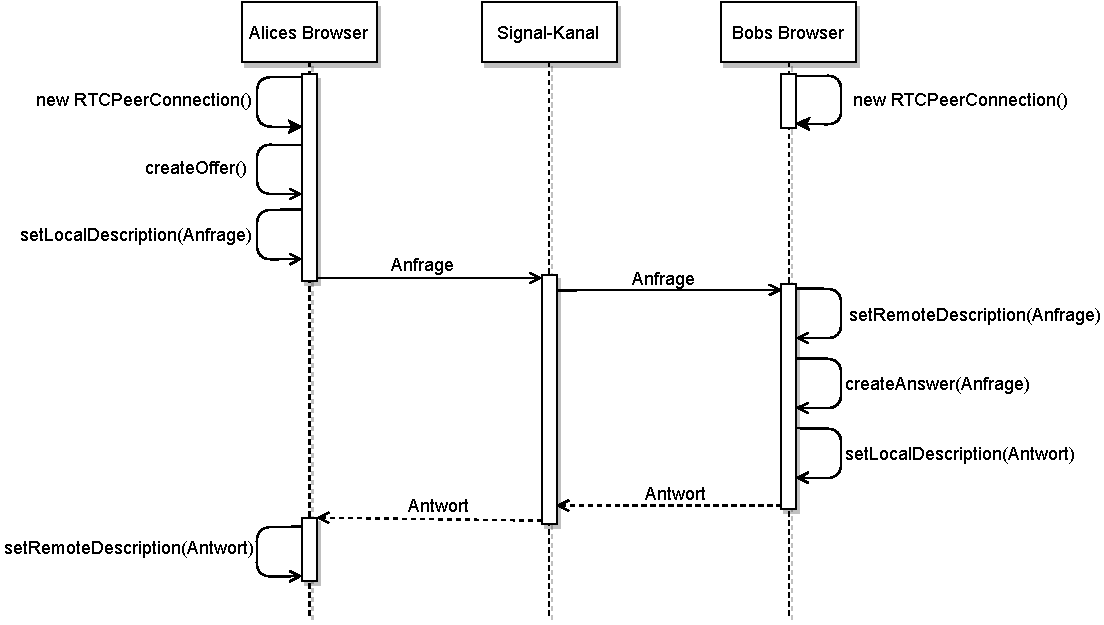
\includegraphics[width=0.95\textwidth]{bilder/PDF_SVG/JSEP.pdf}
\caption{\acs{JSEP}-Verbindungsaufbau.}
\label{fig:jsep}
\end{figure}

\subsubsection{ICE}
\subsubsection{STUN und TURN}
\subsubsection{SCTP}
Zur Übertragung von Daten via RTCDataChannels nutzt \acs{WebRTC} das \acf{SCTP}. Der \acs{SCTP} Standard wurde erstmals im Jahre 2000 von der \acs{IETF} veröffentlicht, und seitdem weiterentwickelt und erweitert. \acs{SCTP} ist ein zuverlässiges, Nachrichtenorientiertes Transportprotokoll, welches im \acf{OSI}-Referenzmodell, ähnlich wie \acs{UDP} oder \acs{TCP}, auf der Transportschicht liegt. Das Protokoll arbeitet dabei basierend auf verbindungslosen Netzwerkprotokollen wie zum Beispiel dem \acf{IP} \cite{sctpRFC}.\par

Im Gegensatz zu \acs{TCP} und \acs{UDP} lassen sich bei \acs{SCTP}, je nach gewünschter Verbindungsart, die folgenden Aspekte unabhängig voneinander frei konfigurieren:
\begin{itemize}
	\item\textbf{Reihenfolge}: \acs{SCTP} ermöglicht es, sowohl geordnete, als auch ungeordnete Datenströme aufzubauen. Falls ein Datenstrom geordnet ist, so müssen die Datenpakete in der Reihenfolge beim Empfänger ankommen, wie sie vom Sender losgeschickt wurden. In ungeordneten Datenströmen ist die Reihenfolge der Pakete, wie sie beim Empfänger ankommen, nicht relevant \cite{sctpRFC}.
	\item\textbf{Zuverlässigkeit}: Die Zuverlässigkeit der Paketlieferungen ist auf zwei Arten konfigurierbar. Es ist möglich, eine maximale Anzahl an Versuchen festzulegen, mit welcher versucht wird, ein Datenpaket zu versenden. Zudem kann eine maximale Lebenszeit für Pakete angegeben werden. Ist diese Lebenszeit, das sogenannte 'Retransmission Timeout' für eine Paketsendung abgelaufen, so wird kein weiterer Versuch unternommen, das Paket abzuschicken \cite{sctpRFC}.
	\item\textbf{Datenströme}: Im Gegensatz zu \acs{TCP} und \acs{UDP} ermöglicht \acs{SCTP} Multiplexing auf Basis von mehreren, separaten sowie parrallelen Datenströmen innerhalb einer Verbindung. Dazu ist der Datenteil eines \acs{SCTP}-Packets in sognenannte \glqq{}Chunks\grqq{}  aufgeteilt, wobei Daten-Chunks jeweils einem Datenstrom zugeordnet werden können \cite{sctpRFC}.
\end{itemize}

\vspace{11pt}

\begin{table}[ht]
\centering
\begin{tabular}[t]{lccc}
\toprule
&TCP&UDP&SCTP\\
\midrule
Nachrichtenordnung&Geordnet&Ungeordnet&Konfigurierbar\\
Zuverlässigkeit&Zuverlässig&Unzuverlässig&Konfigurierbar\\
Datenflusssteuerung&Ja&Nein&Ja\\
Stausteuerung &Ja&Nein&Ja\\
Multihoming&Nein&Nein&Ja\\
Mehrere Datenströme&Nein&Nein&Ja\\
\bottomrule
\end{tabular}
\caption{Vergleich von \acs{TCP} und \acs{UDP} mit \acs{SCTP}.}
\label{table:vergleichNetzwerkProtokolle}
\end{table}

Ein direkter Vergleich der drei Protokolle lässt sich aus Tabelle ~\ref{table:vergleichNetzwerkProtokolle} entnehmen. Im Gegensatz zu \acs{UDP} bietet \acs{SCTP} außerdem Datenfluss- und Stausteuerung. Damit gestaltet sich \acs{SCTP} weitaus flexibler als die beiden gängigsten Transportprotokolle. Zudem ermöglicht \acs{SCTP} Multihoming. Existiert mehr als eine Transportadresse, unter der ein Endpunkt erreicht werden kann, so ist es möglich, im Falle eines Ausfalls des Pfades zum primär verwendeten Endpunkt, Daten über einen weiteren Netzwerkpfad umzuleiten, und an einen weiteren Endpunkt zu verschicken \cite{sctpRFC, multihoming}. Dies erhöht die Zuverlässigkeit der Datenübertragung, und ermöglicht es selbst bei Ausfall eines Netzwerkpfades, Daten weiterhin auszutauschen.\par

\begin{figure}[h]
\centering
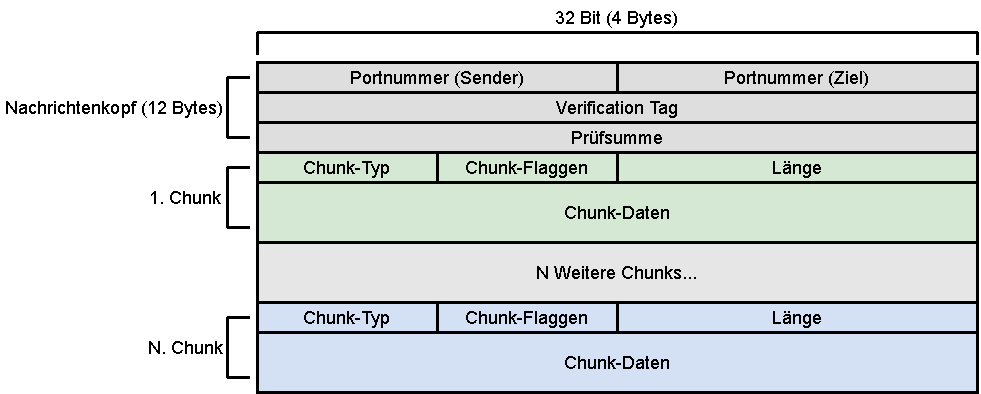
\includegraphics[width=0.95\textwidth]{bilder/PDF_SVG/SCTP_PACKET.pdf}
\caption{Aufbau eines \acs{SCTP}-Packets.}
\label{fig:sctpPacket}
\end{figure}

Ein \acs{SCTP}-Packet besteht aus einem Kopf- und einem Datenteil. Der Kopfteil beinhaltet neben dem Quell- und Zielport, sowie einer Prüfsumme noch ein \glqq{}Verification Tag\grqq{}, welches verwendet wird, um auf der Empfängerseite den Absender des Packets zu verifizieren, und eingehende Packete von denen früherer Verbindungen zu unterscheiden \cite{sctpRFC}.
Der Datenteil des Packets ist in sogenannte \glqq{}Chunks\grqq{}  aufgeteilt. Jedes \glqq{}Chunk\grqq{} besitzt dabei Informationen wie den Chunk-Typ, die Länge in Bytes, oder die Zugehörigkeit zu Datenströmen. Insgesamt existieren über 14 Chunk-Typen, von einfachen Daten-Chunks zu Chunks, welche Daten zur Sitzungskontrolle beinhalten \cite{sctpRFC}. Je nach verwendeten Erweiterungen des \acs{SCTP}-Protokolls kann die Anzahl der Chunk-Typen variieren. Alle Arten dieser \glqq Chunks\grqq{} zu beschreiben würde den Rahmen dieser Arbeit überschreiten. Die generelle Struktur eines Datenpackets ist Abbildung ~\ref{fig:sctpPacket} zu entnehmen. Die maximale größe eines \glqq{}Chunks\grqq{} ist dabei, aufgrund des zwei-Byte langen Längenfelds auf 65,535 Kilobyte limitiert.

\subsubsection{DTLS}

\section{Node.js}
Node.js ist eine kostenlose, plattformunabhängige JavaScript Laufzeitumgebung.
Diese ermöglicht das Ausführen von JavaScript Programmen außerhalb eines Browsers, zum Beispiel auf einem Server. Node.js ist Open-Source und kann kostenlos verwendet werden. Programme setzen sich aus sogenannten \textit{modules}, zu Deutsch Modulen, zusammen. Ein Modul kann dabei jegliche Funktionalität, wie zum Beispiel Klassen, Funktionen und Konstanten exportieren, welche dann wiederrum von weiteren Modulen oder Programmen verwendet werden können. Module können über das \textit{require}-Stichwort geladen werden. Node.js bietet integrierte Webserver-Funktionalität via dem \acs{HTTP}-Modul, welches das Erstellen eines Webservers ermöglicht \cite{nodejs}. Eine JavaScript-Datei kann über den Befehl
\lstset{style=STYLE_COMMAND_LINE_ARGUMENT_SINGLE_LINE}
\begin{lstlisting}[belowskip=-0.8 \baselineskip]
$ node <Pfad zur Skript-Datei>
\end{lstlisting}
ausgeführt werden.\par 

Node.js ist in den Repositories aller aktuellen Linux-Distributionen enthalten\footnote{Weitere Informationen: \url{https://nodejs.org/en/download/package-manager/}}, und kann mit den entsprechenden Packetmanagern, beziehungsweise über die Website\footnote{Node.js Downloads: \url{https://nodejs.org/en/download/}} heruntergeladen und installiert werden.\par

Zur Verwaltung und zum Teilen von Packeten nutzt Node.js den \ac{NPM}. Ein Packet sind in diesem Kontext ein oder mehrere Module, gekoppelt mit allen Dateien, welche diese benötigen. Packete werden auf \textit{npmjs.com} gehostet. Die Liste der von einem Projekt verwendeten Module wird in der Datei \textit{package.json} gespeichert. Ein Packet kann via NPM über den Befehl
\lstset{style=STYLE_COMMAND_LINE_ARGUMENT_SINGLE_LINE}
\begin{lstlisting}[belowskip=-0.8 \baselineskip]
$ npm install <Packetname>
\end{lstlisting}
installiert werden. Ist kein Packetname angegeben, so werden alle Packete, welche im Gleichen Ordner in der \textit{package.json}-Datei eingetragen sind, installiert.

\section{socket.io}
Socket.io ist eine Bibliothek, welche bidirektionale Echtzeitkommunikation zwischen einem Client und einem Server ermöglicht. Dazu nutzt Socket.io intern WebSockets\cite{socketio}. Ein WebSocket ermöglicht Kommunikation zwischen einem Client und einem Server. Der Datenaustausch findet dabei über das \ac{TCP} statt \cite{websocketRFC}. Das WebSocket \ac{API} wird von allen aktuellen Browsern unterstützt\footnote{vgl. \url{https://caniuse.com/mdn-api_websocket}, Stand: 08.04.2021}. Socket.io läuft auf einem Node.js Server\cite{socketio}.\par

Die Kommunikation zwischen Client und Server wird bei Socket.io über Events geregelt. Client und Server können Events -- definiert durch einen String -- mit angehängten Daten emittieren. Basierend auf dem Event-String wird dann auf der Empfängerseite eine Rückruffunktion aufgerufen, vorrausgesetzt diese ist definiert. Die Daten werden der Rückruffunktion als Parameter übergeben. Socket.io ermöglicht auf der Serverseite sowohl das Broadcasting an alle, beziehungsweise an ein Subset an Clients, als auch Unicasting an einen spezifischen Client.\par

Die Socket.io Bibliothek ist in eine Client-, und eine Serverseitige Bibliothek aufgeteilt. Die Clientseitige Bibliothek ermöglicht das Verbinden mit einem Node.js Server. Ein Client kann sowohl Events mit Daten emittieren, als auch Rückruffunktionen registrieren, mit welchen der Client Daten vom Server empfangen kann. Auf der Serverseite ist es möglich, bei Verbindungsaufbau Rückruffunktionen für einen neu verbundenen Client zu registrieren, welche bei dem Eingang von Daten je nach Event-Typ aufgerufen werden. Der Server kann ebenfalls Events an Clients emittieren.

\section{CoTurn STUN / TURN Server}

\section{AWS}